\chapter{DESAIN DAN PERANCANGAN}
  Pada bab ini dibahas mengenai analisis dan perancangan dari sistem. 
  \section{Deskripsi Umum Sistem}    
    Sistem yang akan dibuat adalah sebuah sebuah sistem yang dapat membuat sebuah kontainer \textit{docker} secara otomatis untuk setiap satu \textit{client} yang telah \textit{login} ke dalam sistem. Saat \textit{client} belum \textit{login} ke dalam sistem, maka \textit{client} tersebut akan diarahkan ke halaman \textit{login} dari sistem. Saat \textit{client} mencoba untuk \textit{login} ke dalam sistem, maka sistem akan melakukan pengecekan di dalam basis data apakah \textit{username} dan \textit{password} yang di\textit{input}kan sudah benar atau salah. 
    
    Setelah \textit{client} berhasil \textit{login} ke dalam sistem, sistem akan mengirimkan perintah untuk membuat kontainer \textit{docker} yang berisikan \textit{mitmproxy} ke \textit{docker host}. Setelah berhasil membuat kontainer \textit{docker} untuk client tersebut, maka \textit{traffic} internet dari \textit{client} tersebut akan diarahkan ke kontainer \textit{docker} berisikan \textit{mitmproxy} yang baru saja dibuat. Setelah itu client dapat mengakses internet.
  
  \section{Kasus Penggunaan}
  Terdapat empat aktor dalam sistem yang akan dibuat yaitu \textit{Client}, \textit{Server Login}, \textit{Administrator}, dan \textit{Docker Host}. \textit{Client} adalah aktor yang melakukan proses \textit{login} ke dalam sistem, \textit{server login} adalah aktor yang melakukan proses permintaan penyediaan kontainer \textit{docker}, \textit{administrator} adalah aktor yang melakukan monitoring kontainer \textit{docker} yang sedang berjalan, sedangkan \textit{docker host} adalah aktor yang akan menjadi tempat penyedia kontainer dan menerima perintah penyediaan kontainer. Diagram kasus penggunaan menggambarkan kebutuhan - kebutuhan yang harus dipenuhi sistem. Diagram kasus penggunaan digambarkan pada Gambar \ref{gambarDiagramKasusPenggunaan}.
  \begin{figure}[!h] % h = pasti berada di bawah teks yang ada di atas
  \centering
  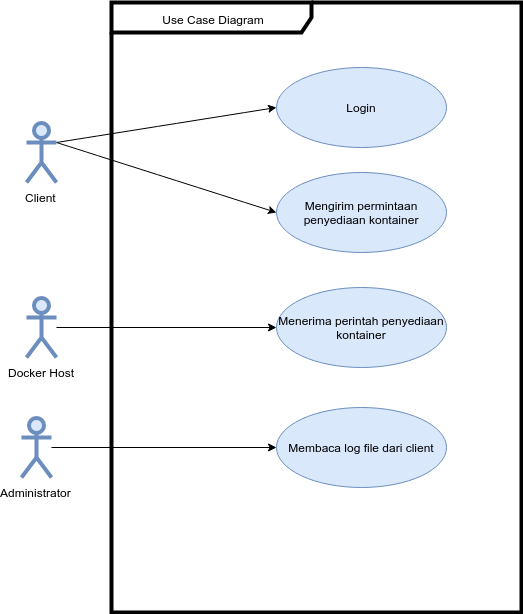
\includegraphics[width=\linewidth]{images/bab3/usecase}
  \caption{Digram Kasus Penggunaan}
  \label{gambarDiagramKasusPenggunaan}
  \end{figure}
  \\
		    		    
	Digram kasus penggunaan pada Gambar \ref{gambarDiagramKasusPenggunaan} dideskripsikan masing-masing pada Tabel \ref{tabelKodeKasusPenggunaan}.
    \begin{longtable}{|p{0.25\textwidth}|p{0.24\textwidth}|p{0.35\textwidth}|} % L = Rata kiri untuk setiap kolom, | = garis batas vertikal.

% Kepala tabel, berulang di setiap halaman
\caption{Daftar Kode Kasus Penggunaan} \label{tabelKodeKasusPenggunaan} \\
\hline
\textbf{Kode Kasus Penggunaan} & \textbf{Nama Kasus Penggunaan} & \textbf{Keterangan} \\ \hline

\endhead
\endfoot
\endlastfoot

% Isi Tabel
UC-0001 & \textit{Login} & \textit{Client} dapat \textit{login} ke dalam sistem. \\ \hline
UC-0002 & Mengirim Permintaan Penyediaan Kontainer \textit{Docker} & \textit{Server login} dapat mengirimkan permintaan penyediaan kontainer \textit{docker} pada \textit{docker host}. \\ \hline
UC-0003 & Menerima Perintah Penyediaan Kontainer \textit{Docker}  &  Proses dimana \textit{docker host} akan menerima perintah dari sistem, untuk menyediakan kontainer secara otomatis.\\ \hline
UC-0004 & Membuat Aturan untuk Mengarahkan \textit{Traffic Client}  &  Proses dimana \textit{docker host} akan membuat aturan untuk mengarahkan \textit{traffic client} ke halaman \textit{login} dari sistem atau untuk membuat aturan untuk mengarahkan \textit{traffic client} ke kontainer \textit{docker} dari tiap-tiap \textit{client}. \\ \hline
UC-0005 & Membaca \textit{Log File} dari \textit{Client}  &  Proses dimana \textit{administrator} dari sebuah jaringan dapat membaca \textit{log file} dari client secara \textit{live} ataupun juga ketika \textit{client} telah selesai menggunakannya.\\ \hline
\end{longtable}

  \section{Arsitektur Sistem}
  	Pada Sub-bab ini, dibahas mengenai tahap analisis arsitektur, analisis teknologi dan desain sistem yang akan dibangun.
    \subsection{Desain Umum Sistem}
      \indent Berdasarkan deskripsi umum sistem yang telah ditulis diatas, dapat diperoleh kebutuhan sistem ini, diantaranya :
        \begin{enumerate}
        \item Pembuatan halaman \textit{login} dari sebuah sistem.
        \item Pembuatan aturan untuk mengarahkan \textit{traffic client} ke halaman \textit{login} dari sistem.
        \item Pembuatan \textit{middleware} untuk menerima permintaan dari \textit{client}.
        \item Pembuatan aturan untuk mengarahkan \textit{traffic client} ke kontainer \textit{docker} dari tiap-tiap \textit{client}.
        \item Pemasangan kontainer pada \textit{docker host}.
        \item Pembacaan \textit{log file} dari \textit{client}.
        \end{enumerate} 
      
      \indent Untuk memenuhi kebutuhan sistem tersebut, penulis membagi sistem menjadi beberapa komponen. Komponen yang akan dibangun antara lain: 
      \begin{enumerate} 
      \item Pembuatan halaman \textit{login} dari sebuah sistem.\\
	      Berfungsi sebagai tampilan antarmuka dari halaman \textit{login} sebuah sistem untuk \textit{client}. Selain itu juga berfungsi untuk mengirimkan permintaan penyediaan kontainer \textit{docker} ke \textit{docker host}.
	  \item Pembuatan aturan untuk mengarahkan \textit{traffic client} ke halaman \textit{login} dari sistem.\\
		  Berfungsi untuk mengarahkan tiap \textit{client} yang belum \textit{login} ke dalam sistem ke halaman \textit{login} dari sistem. Hal ini dilakukan dengan menjalankan sebuah \textit{script} dengan menggunakan \textit{iptables} pada \textit{docker host}.
	  \item Pembuatan \textit{middleware} untuk menerima permintaan dari \textit{client}.
		  Berfungsi untuk menerima permintaan pembuatan kontainer \textit{docker} dari \textit{client}. Selain itu juga berfungsi untuk membuat kontainer \textit{docker} secara otomatis.
	  \item Pembuatan aturan untuk mengarahkan \textit{traffic client} ke kontainer \textit{docker} dari tiap-tiap \textit{client}.\\
		  Berfungsi untuk mengarahkan tiap \textit{client} yang telah berhasil \textit{login} ke kontainer \textit{docker} dari tiap-tiap \textit{client}. Hal ini dilakukan dengan menjalankan sebuah \textit{script} dengan menggunakan \textit{iptables} pada \textit{docker host}.
	  \item Pemasangan kontainer pada \textit{docker host}.\\
		  Berfungsi untuk memasangkan kontainer \textit{docker} pada \textit{docker host} secara otomatis. Hal ini dilakukan dengan menjalankan sebuah perintah penyediaan kontainer pada \textit{docker host}.
	  \item Pembacaan \textit{log file} dari \textit{client}.
		  Berfungsi untuk melihat apa saja yang telak diakses oleh \textit{client}. \textit{Log} yang tersimpan terdapat \textit{log} HTTP maupun \textit{log} HTTPS. Hal ini dilakukan dengan menjalankan sebuah perintah untuk melihat \textit{log file} dari suatu \textit{client}.
        
      \end{enumerate}
      
      \begin{figure}[H]
        \centering
        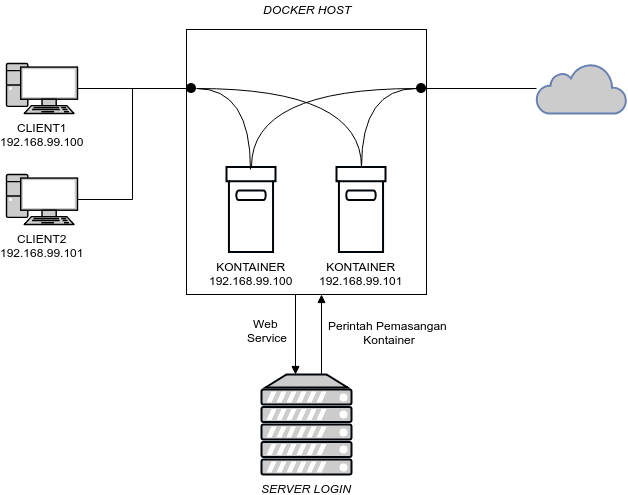
\includegraphics[width=\linewidth]{images/bab3/DIAGRAM1}
        \caption{Arsitektur Komponen Sistem}
        \label{Arsitektur Komponen Sistem}
      \end{figure}
      
    \indent Pada pada Gambar \ref{Arsitektur Komponen Sistem} ditunjukkan arsitektur sistem secara umum dengan detail-detail dari kompenen yang terdapat didalamnya. Setiap komponen tersebut akan diimplementasikan dengan teknologi pendukung yang dibutuhkan.
    
    Nantinya tiap \textit{client}  akan mempunyai satu kontainer \textit{docker} dan satu \textit{port} secara pribadi. \textit{Traffic} dari \textit{client} tersebut akan diarahkan menuju ke kontainer \textit{docker}nya dari tiap-tiap \textit{client}, setelah itu \textit{client} baru dapat mengakses itnernet.
    
    \subsection{Pembuatan halaman \textit{login} dari sebuah sistem.}
    Pembuatan halaman \textit{login} dari sebuah sistem adalah komponen yang bertugas untuk menyediakan tampilan antarmuka dari halaman \textit{login} untuk \textit{client}. Awalnya semua \textit{traffic} diarahkan menuju ke halaman \textit{login} dari sebuah sistem, karena diasumsikan bahwa semua \textit{client} diamsumsikan belum \textit{login} ke dalam sistem. Supaya \textit{client} dapat mengakses internet, maka \textit{client} harus \textit{login} ke dalam sistem terlebih dahulu dengan memasukkan \textit{username} dan \textit{password} dari \textit{client} tersebut.
    
    Dikarenakan ada beberapa kebutuhan yang harus dipenuhi, komponen pada pembuatan halaman \textit{login} dari sebuah sistem dibagi lagi menjadi dua sub komponen, yaitu:
   	\begin{enumerate}
   		\item Basis Data \\
   		Basis data pada komponen pembuatan halaman \textit{login} dari sebuah sistem berfungsi sebagai tempat penyimpanan data \textit{username} dan \textit{password} yang digunakan untuk \textit{login} ke dalam sistem. Basis data juga berfungsi sebagai tempat penyimpanan data kontainer \textit{docker} yang sudah dibuat.
   		\item \textit{Web Service} \\
   		\textit{Web service} berfungsi sebagai antarmuka untuk \textit{client} ketika \textit{client} akan \textit{login} ke dalam sistem. Selain itu \textit{web service} juga berfungsi untuk mengirimkan permintaan penyediaan kontainer \textit{docker} ke \textit{docker host}. Selain itu \textit{web service} juga berfungsi sebagai penerima permintaan dari \textit{client}, yang nantinya akan membuat sebuah kontainer \textit{docker} secara otomatis pada \textit{docker host}.
   	\end{enumerate}
   	
	Pada tugas akhir ini, bahasa Python dipilih sebagai bahasa pemrograman yang digunakan untuk mengimplementasikannya. Lalu, pada bagian penyimpanan data atau basis data, MySQL dipilih sebagai RDBMS untuk tugas akhir ini.
	
	\subsubsection{Desain Basis Data}
	Komponen basis data berfungsi sebagai tempat penyimpanan data \textit{username} dan \textit{password} yang digunakan untuk \textit{login} ke dalam sistem. Dalam basis data ini terdapat satu entitas dan empat atribut, ditunjukkan pada Tabel \ref{tabelnrpmahasiswa}
	\begin{longtable}{|p{0.03\textwidth}|p{0.20\textwidth}|p{0.20\textwidth}|p{0.41\textwidth}|}
		\caption{Atribut basis data nrp-mahasiswa} \label{tabelnrpmahasiswa} \\
		\hline
		\textbf{No} & \textbf{Kolom} & \textbf{Tipe} & \textbf{Keterangan} \\ \hline
		\endhead
		\endfoot
		\endlastfoot
		1 & id & int(11) & Sebagai primary key pada tabel, nilai awal adalah \texttt{AUTO\_INCREMENT}. \\ \hline
		2 & username & varchar(50) & Menunjukkan NRP dari mahasiswa yang telah terdaftar. \\ \hline
		3 & password & varchar(50) & Menunjukkan password dari NRP mahasiswa yang telah terdaftar. \\ \hline
		4 & isLogin & int(11) & Status apakah nrp tersebut sedang digunakan (1), atau sedang tidak digunakan (0). \\ \hline
	\end{longtable}
	
	\subsubsection{Desain \textit{Web Service}}
	Komponen \textit{web service} berfungsi untuk menyediakan antarmuka halaman \textit{login} untuk \textit{client} dan untuk mengirimkan permintaan pembuatan kontainer \textit{docker} secara otomatis pada \textit{docker host} setelah terdapat \textit{client} yang berhasil \textit{login} ke dalam sistem. Halaman \textit{login} akan menggunakan Material UI untuk mendapatkan tampilan yang sederhana dan nyaman untuk digunakan. Desain \textit{web service} untuk halaman \textit{login} dari sistem dapat dilihat pada Gambar \ref{mockuplogin}.
	
	\begin{figure}[H]
		\centering
		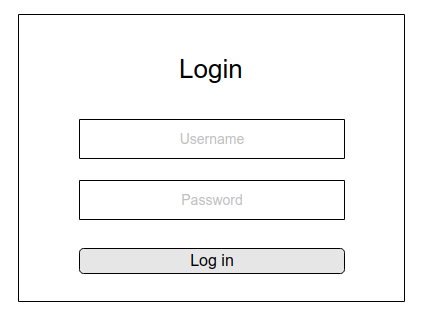
\includegraphics[width=\linewidth]{images/bab3/MockupLogin}
		\caption{Desain Halaman \textit{Login}}
		\label{mockuplogin}
	\end{figure}
	
	Lalu untuk desain \textit{backend} dari \textit{web serive} untuk halaman \textit{login} akan menggunakan bahasa pemrograman Python degan kerangka kerja \textit{flask} yang akan dijalankan dengan \textit{gunicorn}. Kemudian \textit{gunicorn} akan dijalankan dengan \textit{supervisor} sebagai \textit{service}. Lalu akan digunakan \textit{nginx} sebagai \textit{web server} dari halaman \textit{login} dari sebuah sistem. Desain \textit{backend} dari \textit{web service} untuk halaman \textit{login} dapat dilihat pada Gambar \ref{desainbackendhalamanlogin}.
	
	\begin{figure}[H]
		\centering
		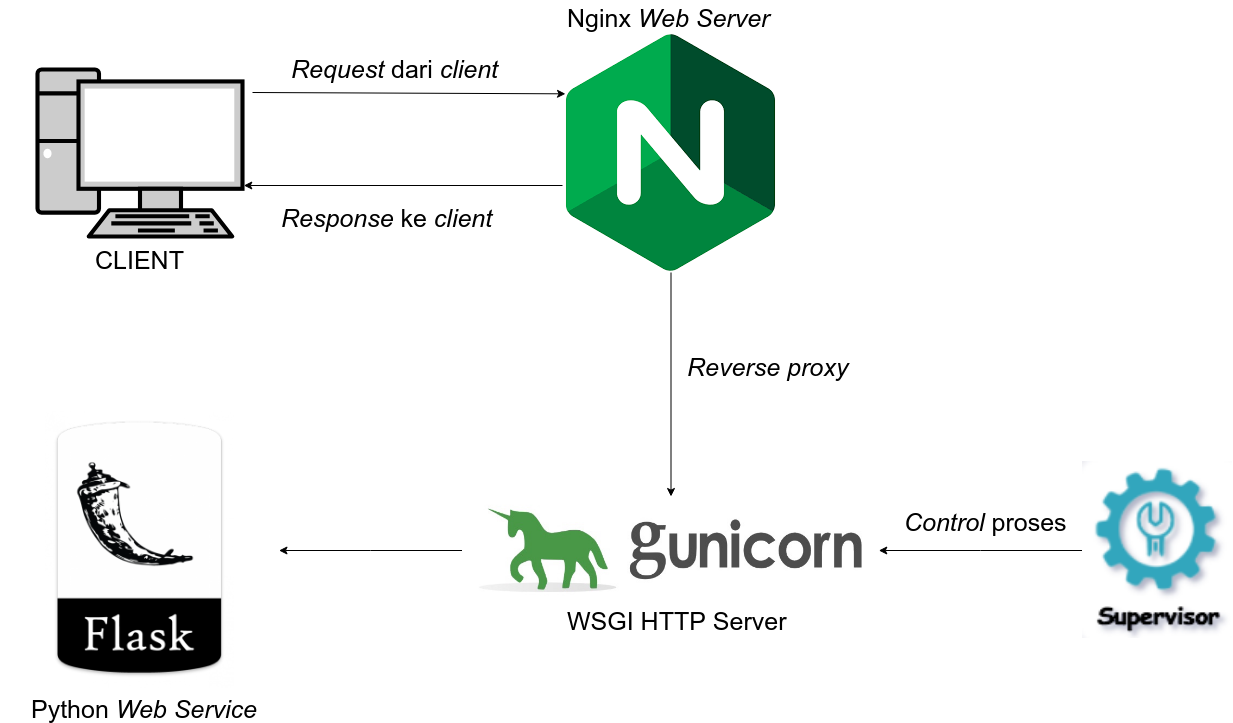
\includegraphics[width=\linewidth]{images/bab3/DesainBackend}
		\caption{Desain \textit{Backend} dari Halaman \textit{Login}}
		\label{desainbackendhalamanlogin}
	\end{figure}
	
	\subsection{Perancangan Pembuatan Aturan untuk Mengarahkan \textit{Traffic Client} ke Halaman \textit{Login} dari Sistem}
	Pembuatan aturan untuk mengarahkan \textit{traffic client} ke halaman \textit{login} dari sistem adalah komponen yang bertugas untuk membelokkan \textit{traffic} dari \textit{client} yang akan menuju ke internet. Awalnya semua \textit{traffic} dari satu \textit{subnet client} tersebut akan diarahkan ke halaman \textit{login} dari sistem dengan membuat sebuah aturan menggunakan \textit{iptables}, karena asumsinya adalah belum ada \textit{client} yang berhasil \textit{login} ke dalam sistem. Desain perancangan pembuatan aturan untuk mengarahkan \textit{traffic client} ke halaman \textit{login} dapat dilihat pada Gambar \ref{dessainmengarahkankehalamanlogin} .
	\begin{figure}[H]
		\centering
		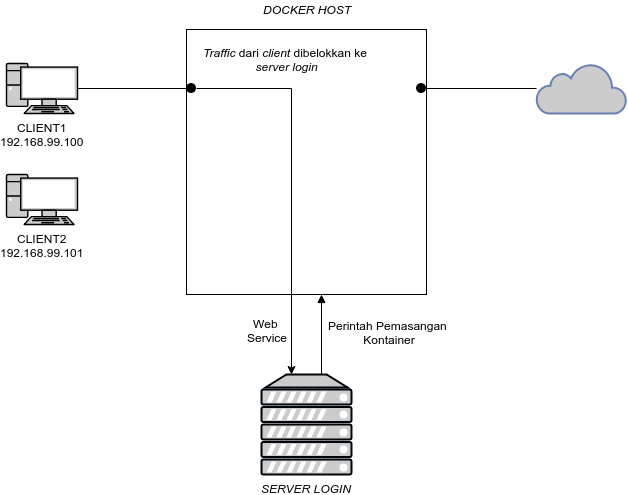
\includegraphics[width=\linewidth]{images/bab3/DIAGRAM2}
		\caption{Desain Mengarahkan \textit{Traffic Client} ke Halaman \textit{Login}}
		\label{dessainmengarahkankehalamanlogin}
	\end{figure}
	
	\subsection{Pembuatan \textit{Middleware} untuk Menerima Permintaan dari \textit{Client}}
	Pembuatan \textit{middleware} untuk menerima permintaan dari \textit{client} adalah komponen yang bertugas untuk menerima permintaan dari \textit{client} yang telah berhasil \textit{login} ke dalam sistem. Permintaan yang dikirimkan oleh \textit{client} adalah permintaan untuk membuat kontainer \textit{docker} secara otomatis. Nantinya setiap satu \textit{client} yang berhasil \textit{login} ke dalam sistem akan dibuatkan satu kontainer \textit{docker}.
	
	Dikarenakan ada beberapa kebutuhan yang harus dipenuhi, komponen pada pembuatan \textit{middleware} untuk menerima permintaan dari \textit{client} dibagi lagi menjadi dua buah komponen, yaitu:
	
   	\begin{enumerate}
   		\item Basis Data \\
   		Basis data  berfungsi sebagai tempat penyimpanan data kontainer \textit{docker} yang sudah dibuat.
   		\item \textit{Web Service} \\
   		\textit{Web service} berfungsi sebagai penerima permintaan dari \textit{client}, yang nantinya akan membuat sebuah kontainer \textit{docker} secara otomatis pada \textit{docker host}.
   	\end{enumerate}
	
	Sama seperti komponen pembuatan halaman \textit{login} dari sebuah sistem, pada tugas akhir ini, bahasa Python dipilih sebagai bahasa pemrograman yang digunakan untuk mengimplementasikannya. Lalu, pada bagian penyimpanan data atau basis data, MySQL dipilih sebagai RDBMS untuk tugas akhir ini. 
	
	\subsubsection{Desain Basis Data}
	Komponen basis data berfungsi sebagai tempat penyimpanan data kontainer \textit{docker} yang sudah dibuat. Dalam basis data ini terdapat satu entitas dan empat atribut, ditunjukkan pada Tabel \ref{tabelkontainer}.
	
	\begin{longtable}{|p{0.03\textwidth}|p{0.20\textwidth}|p{0.20\textwidth}|p{0.41\textwidth}|}
		\caption{Atribut basis data nrp-mahasiswa} \label{tabelkontainer} \\
		\hline
		\textbf{No} & \textbf{Kolom} & \textbf{Tipe} & \textbf{Keterangan} \\ \hline
		\endhead
		\endfoot
		\endlastfoot
		1 & id & int(11) & Sebagai primary key pada tabel, nilai awal adalah \texttt{AUTO\_INCREMENT}. \\ \hline
		2 & username & varchar(50) & Menunjukkan NRP dari mahasiswa yang telah berhasil dibuatkan satu kontainer \textit{docker}. \\ \hline
		3 & ip & varchar(50) & Menunjukkan IP dari \textit{client} yang telah berhasil satu kontainer \textit{docker}. \\ \hline
		4 & createdAt & datetime & Menunjukkan waktu pertama kali kontainer \textit{docker} tersebut dibuat. \\ \hline
		
	\end{longtable}
	
	
	\subsubsection{Desain \textit{Web Service}}
	Komponen \textit{web service} berfungsi untuk menerima permintaan dari \textit{client} untuk membuat satu kontainer \textit{docker} pada \textit{docker host}. Kontainer \textit{docker} yang akan dibuat pada \textit{docker host} akan dibuat secara otomatis oelh sistem, dan kontainer \textit{docker} yang dibuat akan memiliki nama sesuai dengan IP dari \textit{client} yang telah berhasil \textit{login} ke dalam sistem. Setelah menerima permintaan dari \textit{client}, maka sistem akan mengirimkan perintah untuk membuat kontainer \textit{docker} khusus untuk satu \textit{client}. 
   	
    \subsection{Perancangan Pemasangan Kontainer pada \textit{Docker Host}}
	Pemasangan kontainer adalah kompenen yang berfungsi untuk memasangkan kontainer \textit{docker} yang berisikan \textit{mitmproxy} pada \textit{docker host} setelah ada permintaan dari \textit{client} yang telah berhasil \textit{login} ke dalam sistem. Proses ini dilakukan secara otomatis, dan nama dari kontainer \textit{docker} tersebut akan sesuai dengan IP dari \textit{client} yang telah berhasil \textit{login} ke dalam sistem.
	
	Saat kontainer \textit{docker} telah berhasil dibuat, maka kontainer \textit{docker} tersebut akan mempunyai satu port khusus yang sama dengan \textit{client} yang baru saja \textit{login}. Port khusus nantinya akan digunakan untuk mengarahkan \textit{traffic} dari \textit{client} yang akan mengakses internet.
	
	\textit{Image mitmproxy} dipilih sebagai \textit{image} pada kontainer \textit{docker} karena \textit{mitmproxy} merupakan sebuah perangkat lunak yang interaktif dimana \textit{mitmproxy} memungkinkan dapat memotong dan memodifikasi HTTP \textit{requests} atau \textit{response} dengan sangat cepat. \textit{Mitmproxy} sendiri juga dapat berjalan dengan \textit{transparent mode} sehingga \textit{client} tidak mengetahui jika \textit{traffic} dari \textit{client} tersebut ternyata melalui \textit{mitmproxy}. Gambar alur kerja dari \textit{mitmproxy} dengan \textit{transparent mode} untuk HTTP dapat dilihat pada Gambar xx.
	
	\begin{figure}[H]
		\centering
		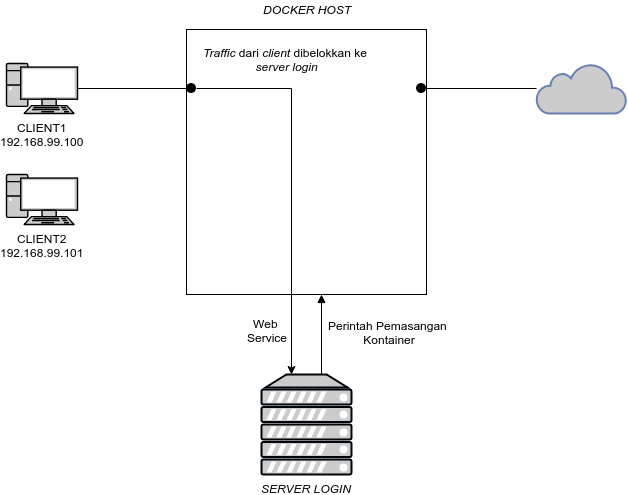
\includegraphics[width=\linewidth]{images/bab3/DIAGRAM2}
		\caption{Desain Mengarahkan \textit{Traffic Client} ke Halaman \textit{Login}}
		\label{dessainmengarahkankehalamanlogin}
	\end{figure}
	
	Sedangkan gambar alur kerja dari \textit{mitmproxy} dengan \textit{transparent mode} untuk HTTPS dapat dilihat pada Gambar xx.
	
	\begin{figure}[H]
		\centering
		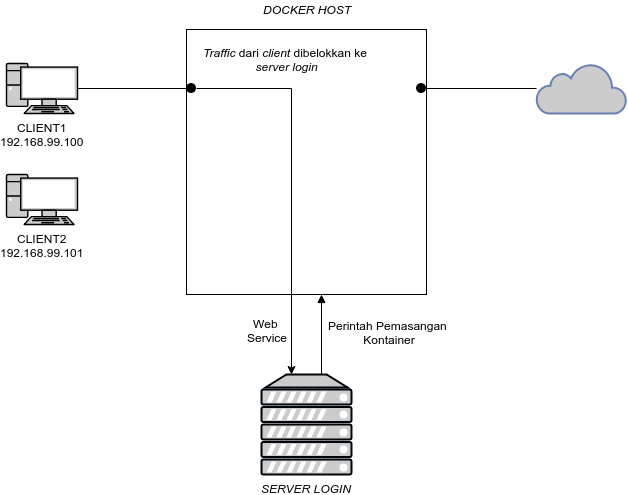
\includegraphics[width=\linewidth]{images/bab3/DIAGRAM2}
		\caption{Desain Mengarahkan \textit{Traffic Client} ke Halaman \textit{Login}}
		\label{dessainmengarahkankehalamanlogin}
	\end{figure}

   	\subsection{Pembuatan Aturan untuk Mengarahkan \textit{Traffic Client} ke Kontainer \textit{Docker} dari Tiap-Tiap \textit{Client}}
   	Pembuatan aturan untuk mengarahkan \textit{traffic client} ke kontainter \textit{docker} dari tiap-tiap \textit{client} adalah komponen yang bertugas untuk mengarahkan satu client ke satu kontainer \textit{docker} yang sesuai. Setelah \textit{client} berhasil \textit{login} ke dalam sistem, maka aturan ini akan dibuat menggunakan \textit{iptables}. Lalu \textit{client} juga akan dibuatkan sebuah aturan dengan menggunakan \textit{iptables} yang memperbolehkan \textit{client} tersebut mengakses internet.